%! TEX root = ../../master.tex
\lecture[Transitive Gruppenwirkungen. Orbit, Stabilisator. Zerlegung von Gruppenwirkungen in Orbite, Isomorphismus mit den Stabilisatornebenklassen. Hauptsatz der Überlagerungstheorie.]{Do 01 Jul 2021}{Hauptsatz der Überlagerungstheorie}

Wir starten mit einem Überblick der letzten Vorlesungen:
\restatetheorem*{AllgemeinerLiftungssatz}

\restatetheorem*{DefCharakteristischeUntergruppe}

\restatetheorem*{ThmHomoeomorpheUeberlagerungen}

\restatetheorem*{ThmKonjugierteCharakteristischeUntergruppen}

\restatetheorem*{ThmUniverselleUeberlagerung}

Insgesamt können wir folgendes zusammenfassen:

\[
    \faktor{\text{zsh. Überlagerungen von $X$}}{\text{Hom über $X$ }} \stackrel{1:1}{\leftrightarrow} \left \{\parbox{14em}{Konjugationsklassen von Untergruppen in $\pi_1(X,x_0)$}\right\} 
\]

\begin{oral}
    Das ganze ist schon sehr toll, aber bisher 'nur' eine mengentheoretische Aussage. Wir würden gerne auch die Homomorphismen (nicht-Isomorphismen insbesondere, die Isomorphismen verstehen wir, zumindest deren Existenz) verstehen.

    Der Hauptsatz der Überlagerungstheorie verfolgt genau dieses Ziel, er gibt eine kategorientheoritschere Verallgemeinerung von obiger Bijektion.
\end{oral}

\begin{definition}
    Eine $G$-Menge  $X$ heißt  \vocab{transitiv}, falls $\forall x,y \in X$ $\exists g\in G$ mit $x.g = y$. 
\end{definition}

\begin{dnotation}
   Wir sagen auch, dass die Wirkung von $G$ auf  $X$ transitiv ist. 
\end{dnotation}

\begin{example}
    Sei $H\subset G$ eine Untergruppe. Dann ist $\cofaktor{H}{G}$, die Menge der Nebenklassen von  $H$, eine transitive  $G$-Menge. Für  $Hg, Hg' \in  \cofaktor{H}{G}$ haben wir nämlich die Wirkung $Hg.(g^{-1}g') = Hg'$.
\end{example}

\begin{lemmadef}[Bahn]\label{def:bahn-orbit}
    Sei $X$ eine  $G$-Menge und  $x\in X$. Dann definiert
    \[
    x.G = \left \{x.g \mid  g\in G\right\} 
    .\] 
    die \vocab{Bahn} oder auch \vocab{Orbit} von $x$. Dann ist  $x.G$ eine Unter- $G$-Menge und  $x.G$ ist transitiv.
\end{lemmadef}
\begin{proof}
    \begin{description}
        \item[Abgeschlossenheit] Sei $x.g \in x.G$ beliebig, dann ist die Wirkung unter einem beliebigen $g'$ genau
            \[
                (x.g).g' = x.(g \circ g')
            .\] 
            in $x.G$ enthalten, weil  $g \circ  g'\in G$.
        \item[Transitivität] Seien $x.g$ und  $x.g'\in x.G$ beliebig. Dann ist
            \[
                (x.g).(gg^{-1}) = x.(gg^{-1}g') = x.g'
            .\] 
            und somit ist die Wirkung transitiv.
    \end{description}
\end{proof}

\begin{lemma}
Sei $X$ eine  $G$-Menge. Seien $x,x' \in X$ beliebig. Dann ist $x.G = x'.G$ oder  $(x.G) \cap  (x'.G) = \emptyset$.
\end{lemma}

\begin{proof}
    Nimm an, dass $(x.G) \cap  (x'.G) \neq  \emptyset$. Wähle also ein $y$ mit 
     \[
         y\in  (x.G) \cap  (x'.G)
    .\] 
    Dann ist also $y = x.g = x'.g'$ für  $g,g' \in G$. Dann ist aber für alle $h\in G$ auch
    \[
        x.h = x.(g.g^{-1}).h = (x.g).g^{-1}.h = y.g^{-1}.h = x'.(g'g^{-1}h) \in x'G
    .\] 
    also ergibt sich $x.G \subset x'G$. Aus Symmetrie folgt $x'.G \subset x.G$, also sind die Klassen gleich.
\end{proof}

\begin{dcorollary}\label{cor:g-menge-ist-disjunkte-vereinigung-der-bahnen}
    Jede $G$-Menge ist die disjunkte Vereinigung ihrer Bahnen.
\end{dcorollary}

\begin{dlemmadef}[Stabilisator]\label{def:stabilisator}
    Sei $X$ eine  $G$-Menge und  $x\in X$. Dann ist der \vocab{Stabilisator} von $x$ die Untergruppe
    \[
    G_x = \left \{g\in G \mid  x.g = x\right\}\leq  G
    .\] 
\end{dlemmadef}
\begin{proof}
    Ist $g\in G_x$, so ergibt sich
    \[
        x = x.e = x.(gg^{-1}) = x.g.g^{-1} = x.g^{-1}
    .\] 
    also ist auch $g^{-1}\in G_x$. Sind zudem $g,h\in G_x$ beliebig, so erhalten wir mit
    \[
        x.(gh) = x.g.h = x.h = x
    .\] 
    auch sofort, dass $gh \in G_x$. Also ist $g_x \leq  G$ tatsächlich eine Untergruppe wie behauptet.
\end{proof}

\begin{lemma}
    Sei $X$ eine  $G$-Menge und  $x\in X$. Dann ist $x.G$ isomorph (als  $G$-Menge) zu  $\cofaktor{G_x}{G}$.
\end{lemma}
\begin{proof}
    Definiere
        \begin{equation*}
        \varphi : \left| \begin{array}{c c l} 
            \cofaktor{G_x}{G} & \longrightarrow & x.G \\
        G_xg & \longmapsto &  x.g
        \end{array} \right.
    \end{equation*}
    \begin{description}
        \item[Wohldefiniertheit] Gleiche Elemente auf der linken Seite unterscheiden sich in ihrer Darstellung nur um ein Element aus $h\in G_x$, wir wollen zeigen, dass dies gleiches Bild ergibt:
            \[
                \varphi (G_xhg) = x.(hg) = x.h.g = x.g = \varphi (G_xg)
            .\] 
        \item[Injektivität] Ist $x.g = x.g'$, dann ergibt sich auch
             \[
            x = x.g'.g^{-1}
            .\] 
            und daraus folgt bereits, dass $g'g^{-1} \in G_x$ nach Definition, also
            \[
                G_xg = G_xg'(g^{-1}g) = G_x(\underbrace{g'g^{-1}}_{\in G_x})g = G_xg'
            .\] 
            also waren auch schon die Nebenklassen gleich.
        \item[Surjektivität] Ist $x.g\in x.G$ beliebig, so ist offensichtlich
            \[
                x.g = \varphi (G_xg)
            .\] 
        \item[$G$-Äquivarianz] (Homomorphismus von $G$-Mengen). Es ist
             \[
                 \varphi ((G_xg)g') = \varphi (G_x(gg')) = x.(gg') = (x.g).g' = \varphi (G_xg).g'
            .\] 
    \end{description}
    Die Mengentheoretische Umkehrabbildung ist dann auch $G$-Äquivariant, also ist  $\varphi $ ein Isomorphismus.
\end{proof}

    \begin{oral}
        Auch, wenn das im Allgemeinen nicht so ist, dass Mengentheorischer Isomorphismus + Kategorientheoretischer Homomorphismus $\implies$ Kategorieller Isomorphismus (das gilt ja z.B. in $\Top$ nicht, siehe  $\exp \colon  [0,1) \to  S^1$), gilt dies für $G$-Mengen (und im Übrigen auch für Gruppen).
    \end{oral}

    Also ist jede $G$-menge isomorph zu einer disjunkten Vereinigung um $G$-Mengen der Form $\cofaktor{H}{G}$, wobei  $H\leq G$.

\begin{warning}
    Auch, wenn wir die Notation $\cofaktor{H}{G}$ verwendet haben, wollen wir damit nicht notwendigerweise ausdrücken, dass  $H$ normal ist in  $G$, wir haben nur die Menge der Nebenklassen betrachtet, und zwar als Menge.
\end{warning}

\section{Hauptsatz der Überlagerungstheorie}

Sei in diesem Kapitel stets $p\colon  E\to X$ eine Überlagerung.

\begin{lemmadef}
    Die Gruppe $\pi_1(X,x_0)$ wirkt folgendermaßen auf $p^{-1} (x_0)$: Sei $e\in p^{-1} (x_0)$, und $[w]\in \pi_1(X,x_0)$, dann definiere
    \[
        e.[w] = L(w,e)(1) \in p^{-1} (x_0)
    .\] 
    Mit dieser Wirkung ist $p^{-1} (x_0)$ eine $G$-Menge.
\end{lemmadef}
\begin{proof}
    \begin{description}
        \item[Wohldefiniertheit] Sind $w,w'$ homotop relativ Endpunkten sind, dann auch  $L(w,e)$ und  $L(w',e)$ nach dem \nameref{thm:homotopieliftungssatz}, also sind insbesondere ihre Endpunkte gleich.
        \item[Axiome der Gruppenwirkung] Es ist offenbar
            \[
                e.[c_{x_0}] = L(c_{x_0},e) = c_{e}(1) = e
            .\] 
            und auch 
            \begin{IEEEeqnarray*}{rCl}
                e.([w] \star [w]) & = & L(w \star w,e)(1) \\
                                  & = & (L(w,e)\star L(w',L(w,e)(1)))(1) \\
                                  & = & L(w',\underbrace{L(w,e(1)}_{= e.[w]})(1) \\
                                  & = & (e.[w]).[w']
            \end{IEEEeqnarray*}
    \end{description}
\end{proof}

\begin{oral}
    An dieser Stelle geht das einzige Mal ein, dass wir links-$G$-Mengen betrachtet haben, weil wir die Verknüpfung von Schleifen in dieser Richtung definiert hatten.
\end{oral}

\begin{lemma}
    Sind $p\colon  E\to X$ und $p'\colon E'\to X$ Überlagerungen sowie $x_0\in X$. Sei $f\colon  E\to  E'$ eine Abbbildung von Überlagerungen, d.h. $p = p' \circ f$. Dann ist
    \[
        f|_{p^{-1} (x_0)}\colon  p^{-1} (x_0) \to  p'^{-1}(x_0)
    .\] 
    ein Homomorpismus von $\pi_1(X,x_0)$-Mengen.
\end{lemma}
\begin{proof}
    \begin{description}
        \item[Wohldefiniertheit] Sei $e\in p^{-1} (x_0)$. Dann ist $p'(f(e)) = p(e) = x_0$, also ist $f(e) \in p^{-1} (x_0)$.
        \item[Äquivarianz] Sei $e\in p^{-1} (x_0)$ sowie $[w]\in \pi_1(X,x_0)$ beliebig. Dann ist
            \[
                f(e).[w] = L_{p'}(w,f(e))(1) \stackrel{!}{=} f \circ L_p(w,e)(1) = f(e.[w])
            .\] 
            Das ergibt sich aber, indem wir nachrechnen, dass $f \circ  L_p(w,e)$ \textit{eine} Liftung ist, denn
            \[
                p' \circ  f \circ  L_p(w,e) = p \circ  L_p(w,e) = w
            .\]
            aber mittlerweile ist uns klar, dass Liftungen eindeutig sind nach dem \nameref{thm:weghebungssatz}.
    \end{description}
\end{proof}

\begin{lemma}\label{lm:funktor-von-überlagerungen-in-pi-1-mengen}
    Die Zuordnung
    \begin{IEEEeqnarray*}{cCc}
        \text{Überlagerungen von $X$} &\longrightarrow &\pi_1(X,x_0)\text{-Mengen} \\ \\
    \begin{tikzcd}
        E \ar{d}{p} \\ X
    \end{tikzcd}
    \qquad&    \longmapsto  & \qquad p^{-1} (x_0) \\ \\
    \begin{tikzcd}[column sep = tiny]
    E \ar{rr}{f} \ar[swap]{dr}{p} & & E' \ar{dl}{p'} \\
    & X
\end{tikzcd} \qquad & \longmapsto &  \qquad     f|_{p^{-1} (x_0)}: p^{-1} (x_0) \to  p'^{-1}(x_0)
    \end{IEEEeqnarray*}
    ist ein Funktor.
\end{lemma}
\begin{proof}
    Wir haben schon gezeigt, dass das eine Wohldefinierte Zuordnung (Abbildung) ist. Wir müssen noch zeigen, dass das ganze mit Verknüpfung verträglich ist, und Identitäten auf Identitäten gehen. Ist also
    \[
    \begin{tikzcd}[column sep = tiny]
    E' \ar{rr}{g} \ar[swap]{dr}{p'} & & E'' \ar{dl}{p''} \\
    & X
    \end{tikzcd}
    \]
    ein weiterer Morphismun von Überlagerungen, so ist
    \[
        (g \circ f)|_{p^{-1} (x_0)} = g|_{p^{-1} (x_0)}  \circ  f|_{p^{-1} (x_0)}
    .\] 
    und es ist sicherlich auch
    \[
        (\id_E)|_{p^{-1} (x_0)} = \id_{p^{-1}(x_0)}
    .\] 
    also erfüllt diese Abbildung die Eigenschaften eines Funktors.
\end{proof}


\begin{restatable}[Hauptsatz der Überlagerungstheorie]{theorem}{ThmHauptsatzUeberlagerungstheorie}\label{thm:hauptsatz-der-überlagerungstheorie}
    Sei $X$ zusammenhängend, lokal wegzusammenhängend, semilokal einfachzusammenhängend sowie  $x_0\in X$. Dann ist der Funktor aus \autoref{lm:funktor-von-überlagerungen-in-pi-1-mengen} eine Äquivalenz von Kategorien. Das heißt:
    \begin{enumerate}[1)]
        \item Für jede $\pi_1(X,x_0)$-Menge $M$ gibt es eine Überlagerung  $p\colon  E \to X$, so dass $p^{-1} (x_0)$ isomorph ist (als $\pi_1(X,x_0)$-Menge) zu  $M$. (\textit{essentielle Surjektivität})
        \item Für zwei Überlagerungen $p\colon  E \to X$ und $p' \colon  E' \to  X$ ist die Zuordnung
            \begin{IEEEeqnarray*}{cCc}
                \left\{
                    \begin{tikzcd}[column sep = tiny, ampersand replacement = \&]
                E \ar{rr}{f} \ar[swap]{dr}{p} \& \& E' \ar{dl}{p'} \\
                \& X
        \end{tikzcd}\right\} & \longmapsto & \left \{f|_{p^{-1} (x_0)\colon  p^{-1} (x_0) \to  p'^{-1}(x_0)}\right\} 
            \end{IEEEeqnarray*}
    \end{enumerate}
\end{restatable}

\begin{oral}
    Für die 'Entpackung' dieser kategorientheoretischen Aussage haben wir die Charakterisierung von TODO.
\end{oral}

\begin{remark}
    Die Eigenschaft, dass $X$ semilokal einfachzusammenhängend ist, benötigen wir nur für Eigenschaft 1), um z.B. eine universelle Überlagerung konstruieren zu können. Für 2) genügt es allerdings zu fordern, dass  $X$ zusammenhängend und lokal wegzusammenhängend ist.
\end{remark}

\begin{remark*}
    An dieser Stelle haben wir nun \nameref{thm:seifert-van-kampen} eingeführt, und weite Teile von \autoref{sec:seifert-van-kampen} vorgezogen, damit diese vor der Klausur bekannt sind. Erst danach sind wir hierher zurückgekommen, und haben den \nameref{thm:hauptsatz-der-überlagerungstheorie} bewiesen. 
\end{remark*}

\lecture[Bijektion zwischen Orbits und Wegekomponenten. Morphismen von transitiven $g$-Mengen. Alternativer Beweis des Isomorphismus  $\Delta(p) \cong \cofaktor{H}{N_{\pi_1(X,x_0)}H}$.]{Do 08 Jul 2021}[22]{Beweis des Hauptsatzes der Überlagerungstheorie}

Wir erinnerns uns daran, dass die Wirkung von $\pi_1(X,x_0)$ auf $p^{-1} (x_0)$ durch
\[
    e.[w] \coloneqq  L(w,e)(1)
.\] 
gegeben ist.

\begin{proposition}\label{prop:wegekomponenten-von-überlagerungsraum-sind-bahnen-von-faser-bezüglich-fundamentalgruppe-wenn-basisraum-wegzusammenhängend}
    Sei $p\colon E\to X$ eine Überlagerung,  $X$ wegzusammenhängend sowie  $x_0\in X$. Dann induziert die Inklusion $p^{-1} (x_0) \hookrightarrow E$ eine Bijektion
    \[
        \left \{\pi_1(X,x_0) - \text{Bahnen von } p^{-1} (x_0) \right\}  \stackrel{1:1}{\longleftrightarrow} \left \{\text{Wegekomponenten von } E\right\} 
    .\] 
\end{proposition}

\begin{proof}
    \begin{description}
        \item[Wohldefiniertheit] Zu zeigen: Für $e\in p^{-1} (x_0)$ liegen $e$ und  $e.[w]$ in der gleichen Wegekomponente. Es ist aber
             \[
                 e.[w] = L(w,e)(1)
            .\] 
            und damit ist $L(w,e)$ ein Weg von  $e$ nach  $e.[w]$, und somit liegen die Punkte in der gleichen Wegekomponenten von  $E$.
        \item[Injektivität] Seien  $e,e'\in p^{-1} (x_0)$, so dass diese auf die gleiche Wegkomponenten abgebildet werden, dann gibt es einen Weg $v$ von  $e$ nach  $e'$. Dann ist
             \[
                 e.\underbrace{[p \circ  v]}_{\in \pi_1(X,x_0)}  = L(p \circ  v, e)(1) = v(1) = e'
            .\] 
            also liegen $e,e'$ in der gleichen Bahn.
        \item[Surjektivität] Sei  $\tilde{E}$ eine Wegekomponente von $E$ sowie  $e\in \tilde{E}$. Aufgrund des Wegzusammenhangs von $X$ finden wir einen Weg  $v$ von  $p(e)$ nach  $x_0$. Dann ist $L(v,e)$ ein Weg von  $e$ mit Endpunkt in  $p^{-1} (x_0)$, also $\tilde{E} \cap  p^{-1} (x_0) \neq  \emptyset$.
    \end{description}
\end{proof}

Ist $e\in p^{-1} (x_0)$, so ist der Orbit
\[
    e.\pi_1(x,x_0) \cong_{\pi_1(X,x_0)-\text{Menge}} \cofaktor{\pi_1(X,x_0)_e}{\pi_1(X,x_0)}
.\] 

Also interessieren wir uns auch für Elemente aus dem Stabilisator $\pi_1(x,x_0)_e$. Hierzu ist
\[
    e.[w] = e \iff  L(w,e)(1) = e \iff  L(w,e) \text{ ist Schleife an } e \iff  [w] \in  p_*(\pi_1(E,e))
.\] 

Also ist $e.\pi_1(X,x_0) \cong \cofaktor{p_*(\pi_1(E,e))}{\pi_1(X,x_0)}$.

\begin{proof}[Beweis von \autoref{thm:hauptsatz-der-überlagerungstheorie}]
    \underline{1. Schritt} Wir zeigen die essentielle Surjektivität. Sei $M$ eine  $\pi_1(X,x_0)$-Menge. Dann ist $M$ isomorph zu einer disjunkten Vereinigung
    \[
        M = \bigsqcup_{i\in I} \cofaktor{H_i}{\pi_1(X,x_0)}
    .\] 
    Mit $H_i \leq  \pi_1(X,x_0)$. Nach \autoref{thm:universelle-überlagerungen-existieren-genau-für-semilokal-einfachzusammenhängende-lokal-wegzusammenhängenden-zusammenhängende-räume} existieren Räume $E(H_i)$, sodass
     \[
         p(H_i) \colon  E(H_i) \to  X
    .\] 
    sowie $e_i\in p(H_i)^{-1}(x_0)$ mit 
    \[
        p(H_i)_* \pi_1(E(H_i),e_i) = H_i
    .\] 
    Dann ist $p(H_i)^{-1}(x_0)$ isomorph zu $\cofaktor{H_i}{\pi_1(X,x_0)}$ nach \autoref{prop:wegekomponenten-von-überlagerungsraum-sind-bahnen-von-faser-bezüglich-fundamentalgruppe-wenn-basisraum-wegzusammenhängend} und der Vorüberlegung. Wir betrachten nun die disjunkte Vereinigung
    \[
        p\coloneqq  \coprod p(H_i) \colon  \coprod _{i \in I} E(H_i) \to  X
    .\] 
    so ist
    \[
        p^{-1} (x_0) = \bigsqcup p(H_i)^{-1}(x_0) \cong \coprod_{i \in I} \cofaktor{H_i}{\pi_1(X,x_0)} \cong M
    .\] 
    \begin{remark}
        Es fehlt noch zu zeigen, dass $p$ überhaupt eine Überlagerung ist, im allgemeinen ist das Koprodukt von Überlagerungen nämlich \textit{nicht} zwingend wieder eine Überlagerung. Wir müssen das also in diesem konkreten Fall noch zeigen.
    \end{remark}
    \begin{claim}
        Sei $x\in X$ und $x\in U\subset X$ eine wegzusammenhängende Umgebung mit $\pi_1(U) \to  \pi_1(X)$ trivial. Dann ist $U$ eine trivialisierende Umgebung für alle  $p(H_i)$ und damit auch für  $p$.
    \end{claim}
    \begin{subproof}
        Folgt unmittelbar aus der Konstruktion, die wir gewählt hatten, denn wir haben gezeigt, dass die trivialisierenden Umgebungen genau diejenigen Basiselement von $X$ aus  \autoref{lm:basis-vonsemilokal-einfachzusammenhängendem-zusammenhängendem-raum} sind, und diese waren unabhängig von der Überlagerung.
    \end{subproof}
    \underline{2. Schritt} Wir zeigen die volltreue.

    \underline{Injektivität} Seien $f,\hat{f}$ zweie Überlagerungsabbildungen, d.h.
    \[
    \begin{tikzcd}[column sep = tiny]
        E \ar{rr}{f}[swap]{\hat{f}} \ar[swap]{dr}{p} & & E' \ar{dl}{p'} \\
    & X
    \end{tikzcd}
    \]
    die unter dem Funktor das gleiche Bild haben, d.h. $f|_{p^{-1} (x_0)} = \hat{f}|_{p^{-1} (x_0)}$. Wir wollen zeigen, dass dann auch schon $f \equiv  \hat{f}$. Sei $\tilde{E} \subset E$ eine beliebige Wegekomponenten. Es genügt zu zeigen, dass $f|_E = \hat{f}|_{\tilde{E}}$.

    Da $X$ lokal wegzusammenhängend ist  $p|_{\tilde{E}}\colon \tilde{E} \to  X$ bereits eine Überlagerung nach \autoref{thm:überlagerung-über-lokal-wegzusammenhängendem-raum-zerfällt-in-wegzusammenhängende-komponenten-von-e}.

    Es ist $\tilde{E} \cap  p^{-1} (x_0) \neq  \emptyset$. Sei $e\in \tilde{E} \cap  p^{-1} (x_0)$. Dann sind $f|_{\tilde{E}}$ und $\hat{f}|_{\tilde{E}}$ Hebungen von
    \[
        \begin{tikzcd}[column sep = large, row sep = large]
        & E' \ar{d}{p'} \\
        \tilde{E} \ar[shift left]{ur}{f|_{\tilde{E}}} \ar[shift right, swap]{ur}{\hat{f}|_{\tilde{E}}} \ar{r}{p|_{\tilde{E}}} & X
    \end{tikzcd}
    .\] 

    \underline{Surjektivität}. Sei $\tilde{f} \colon  p^{-1} (x_0) \to  p'^{-1}(x_0)$ ein Homomorphismus von $\pi_1(X,x_0)$-Mengen. Wir möchten zeigen, dass dieser auch schon von einer Überlagerungsabbildung $f\colon  E \to  E'$ induziert wird. 

    Sei wieder $\tilde{E} \subset E$ eine Wegekomponente, dann ist $p^{-1} (x_0) \cap \tilde{E}$ genau eine Bahn von $p^{-1} (x_0)$ nach ebiger Proposition.

    Sei $e\in p^{-1} (x_0) \cap \tilde{E}$, dann ist
    \[
        p^{-1} (x_0) \cap  \tilde{E} \cong \cofaktor{\underbrace{p_*(\pi_1(E,e))}_{\coloneqq H}}{\pi_1(X,x_0)}
    .\] 
    nach der Vorüberlegung. Es ist $\tilde{f}(e) \in p'^{-1}(x_0)$.

    \begin{claim}
        Es ist $H\leq  p_*'(\pi_1(E',\tilde{f}(e)))$.
    \end{claim}
    \begin{subproof}
        Sei $h\in H$. Dann ist gerade
        \[
            \tilde{f}(e).  h = \tilde{f}(e.h) = \tilde{f}(e) \implies h\in \pi_1(x,x_0)_{\tilde{f}(e)}
        .\] 
        Also ergibt sich
        \[
            H \leq  \pi_1(X,x_0)_{\tilde{f}(e)} = p_*'(\pi_1(E',\tilde{f}(e)))
        .\] 
    \end{subproof}

    Nach dem \nameref{thm:allgemeiner-liftungssatz} existiert also eine Abbildung $f|_{\tilde{E}}\colon \tilde{E} \to  E'$ mit $f|_{\tilde{E}}(e) = \tilde{f}(e)$.
    \[
    \begin{tikzcd}
        & E \ar{d}{p'} \\
        \tilde{E} \ar[dashed]{ur}{f|_{\tilde{E}}} \ar[swap]{r}{p|_{\tilde{E}}} & X
    \end{tikzcd}
    .\]
    \begin{claim}
        Es gilt nun sogar 'automatisch' $f|_{\tilde{E}}(e') = \tilde{f}(e')$ für alle $e' \in p^{-1} (x_0) \cap  \tilde{E}$.
    \end{claim}
    \begin{subproof}
        Mit \autoref{cor:f-und-f-til-sind-gleich-im-hauptsatz}  nach der Pause.
    \end{subproof}
    Definiere nun $f\colon  E \to  E'$ durch
    \[
    E = \coprod \tilde{E} \stackrel{\coprod f|_{\tilde{E}}}{\longrightarrow} E'
    .\] 
    Dann ist $f|_{p^{-1} (x_0)} = \tilde{f}$ nach ebiger Behauptung.
\end{proof}


\begin{lemma}\label{lm:morphismus-von-g-mengen-von-transitiver-menge-ist-auf-einem-element-bestimmt}
    Sei $G$ eine Gruppe,  $M$ eine transitive  $G$-Menge.  $N$ eine  $G$-Menge,  $m\in M$ und $\varphi ,\varphi '\colon M \to  N$ Morphismen von $G$-Mengen. Dann ist bereits $\varphi  \equiv  \varphi '$.
\end{lemma}
\begin{proof}
    Sei $m' \in M$ beliebig. Wegen Transitivität existiert $g\in G$ mit $m.g = m'$. Also rechnen wir einfach nach:
     \[
         \varphi (m') = \varphi (m.g) = \varphi (m).g = \varphi' (m).g = \varphi' (m.g) = \varphi '(m')
    .\] 
\end{proof}

\begin{corollary}\label{cor:f-und-f-til-sind-gleich-im-hauptsatz}
    Es gilt $f|_{\tilde{E}}(e') = \tilde{f}(e')$ für alle $e'\in p^{-1} (x_0) \cap  \tilde{E}$.
\end{corollary}

\begin{proof}
    Folgt als Spezialfall von \autoref{lm:morphismus-von-g-mengen-von-transitiver-menge-ist-auf-einem-element-bestimmt} mit $G = \pi_1(X,x_0)$, $M = p^{-1} (x_0) \cap \tilde{E}$, $N = p'^{-1}(x_0)$ sowie $m = e$ und 
     \[
         \varphi  = (f|_{\tilde{E}})|_{p^{-1} (x_0)\cap \tilde{E}} \qquad \varphi ' = \tilde{f}|_{p^{-1} (x_0) \cap \tilde{E}}
    .\] 
\end{proof}

Damit ist nun der Beweis von \autoref{thm:hauptsatz-der-überlagerungstheorie} abgeschlossen.

Wir erinnerns uns kurz an:

\restatetheorem*{LmDecktransformation}

\restatetheorem*{ThmDecktransformationNormalisator}

und an den verbundenen \autoref{thm:isomorphismus-von-decktransformationen-mit-nebenklassengruppe-von-charakteristischer-untergruppe-in-seinem-normalisator}.


\begin{minipage}{\textwidth}
    \centering
    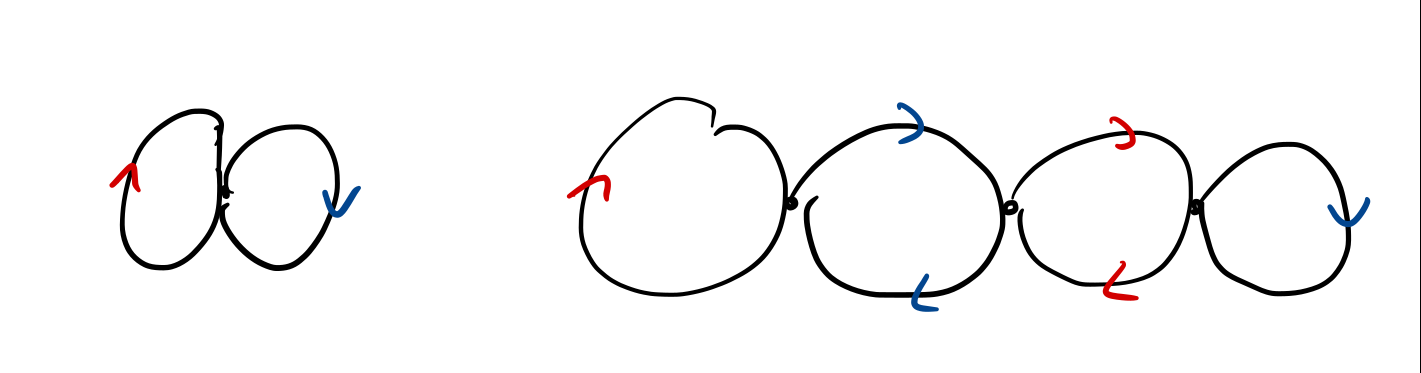
\includegraphics[scale=0.25]{figures/handdrawn/skizze-nach-19.3}
    \captionof{figure}{Eine Überlagerung von $S^1 \twedge S^1$}
\end{minipage}

Mit dem \autoref{thm:hauptsatz-der-überlagerungstheorie} ergibt sich nun der folgende Alternative Beweis:

\begin{proof}[Alternativer Beweis von \autoref{thm:isomorphismus-von-decktransformationen-mit-nebenklassengruppe-von-charakteristischer-untergruppe-in-seinem-normalisator}]
    
    Es sind $\Delta(p)$ genau die Automorphismen der Überlagerung  $p\colon  E \to X$. Nach dem Hauptsatz sind diese also isomorph zu den Automorphismen von $p^{-1} (x_0)$ als $\pi_1(X,x_0)$-Mengen, die wiederum isomorph sind zu den Automorphismen von $\cofaktor{p_*(\pi_1(E,e_0))}{\pi_1(X,x_0)}$, d.h.
\[
    \Delta(p) = \Aut \left(
    \begin{tikzcd}
        E \ar{d}{p} \\ X
    \end{tikzcd}\right) 
    \cong \Aut_{\pi_1(X,x_0)-\text{Mengen}} (p^{-1} (x_0)) \cong \Aut \left( \cofaktor{p_*(\pi_1(E,e_0)}{\pi_1(x,x_0)} \right) 
.\] 
\end{proof}

\begin{proposition}
    Es ist
    \[
        \Aut_{G-\text{Mengen}}\left(\cofaktor{H}{G}\right) \cong \cofaktor{H}{N_GH}
    .\] 
\end{proposition}
\begin{proof}
    Sei $f\colon  \cofaktor{H}{G} \to  \cofaktor{H}{G}\in \Aut \left(\cofaktor{H}{G}\right)$ ein solcher Automorphismus.
    \begin{enumerate}[1)]
    \item Dann ist $f$ bereits eindeutig bestimmt durch  $f(H)$ nach \autoref{lm:morphismus-von-g-mengen-von-transitiver-menge-ist-auf-einem-element-bestimmt}.
    \item $f(H.1) \in \cofaktor{H}{N_GH}$. ist $f(H.1) = H.g_0$, dann ist für alle $h\in H$ auch $H.g_0 = f(H.1) = f(H.h) = f(H.1).h = H.g_0.h$.

        Daraus folgt bereits, dass $\exists h_1,h_1 \in H$ mit $h_1g_0 = h_2g_0h$, also nach umformen
        \[
       h_2^{-1}h_1 = g_0hg_0^{-1}
        .\] 
        wegen $h\in H$ beliebig ergibt sich also bereits $g_0Hg_0^{-1}\subset H$. Das Inverse schickt $Hg_0$ auf $H$. Also schickt se  $H$ auf  $Hg_0^{-1}$. Analog zeigen wir, dass $g_0^{-1}Hg_0 \subset H$, also auch $H\subset g_0Hg_0^{-1}\subset H$ und somit schlussendlich
        \[
        H = g_0Hg_0^{-1} \qquad \implies \qquad g_0\in N_GH
        .\] 
        Die Abbildung
        \[
            f \mapsto f(H\cdot 1)
        .\] 
        ist also wohldefiniert und injektiv nach 1)

    \item Wir zeigen noch Surjektivität. Ist $g_0\in N_GH$, so behaupten wir, dass
        \[
        Hg \mapsto Hg_0g
        .\] 
        wohldefiniert und $G$-äquivariant ist. Die Äquivarianz ist nach Definition offensichtlich. Für Wohldefiniertheit bilden wir ab
         \[
             Hhg \mapsto H g_0hg \stackrel{g_0\in N_GH}{=} H h'g_0g = Hg_0g
        .\] 
        Da $N_GH$ eine Untergruppe ist, ist auch  $g_0^{-1}\in N_GH$, also hat die Abbildung ein Inverses, und zwar
        \[
        Hg \mapsto Hg_0^{-1}g
        .\] 
\end{enumerate}
\end{proof}
